\documentclass[Rapport/Rapport_main.tex]{subfiles}
\begin{document}
\subsection{Database}
Databasen skal agerer som et filsystem til lagring af brugerinformation, samt interaktioner mellem brugere i form af et beskedsystem. Til dette formål designes en relationel database, som skal opbevare applikationens data og være fælles opbevaringstjeneste for alle brugere i systemet. Det skal være muligt at tilgå data og samtidigt opretholde dataets integritet. Databasen skal være serverbaseret, og vil bruges som et kommunikationssystem mellem brugere. \\\\
Databasen er designet ud fra relationalmodellen af data, hvor relationer kan sammenlignes med hinanden. Systemets data- og informationsstruktur defineres i E/R diagrammet set nedenfor. 
\begin{figure}[H]
    \centering
    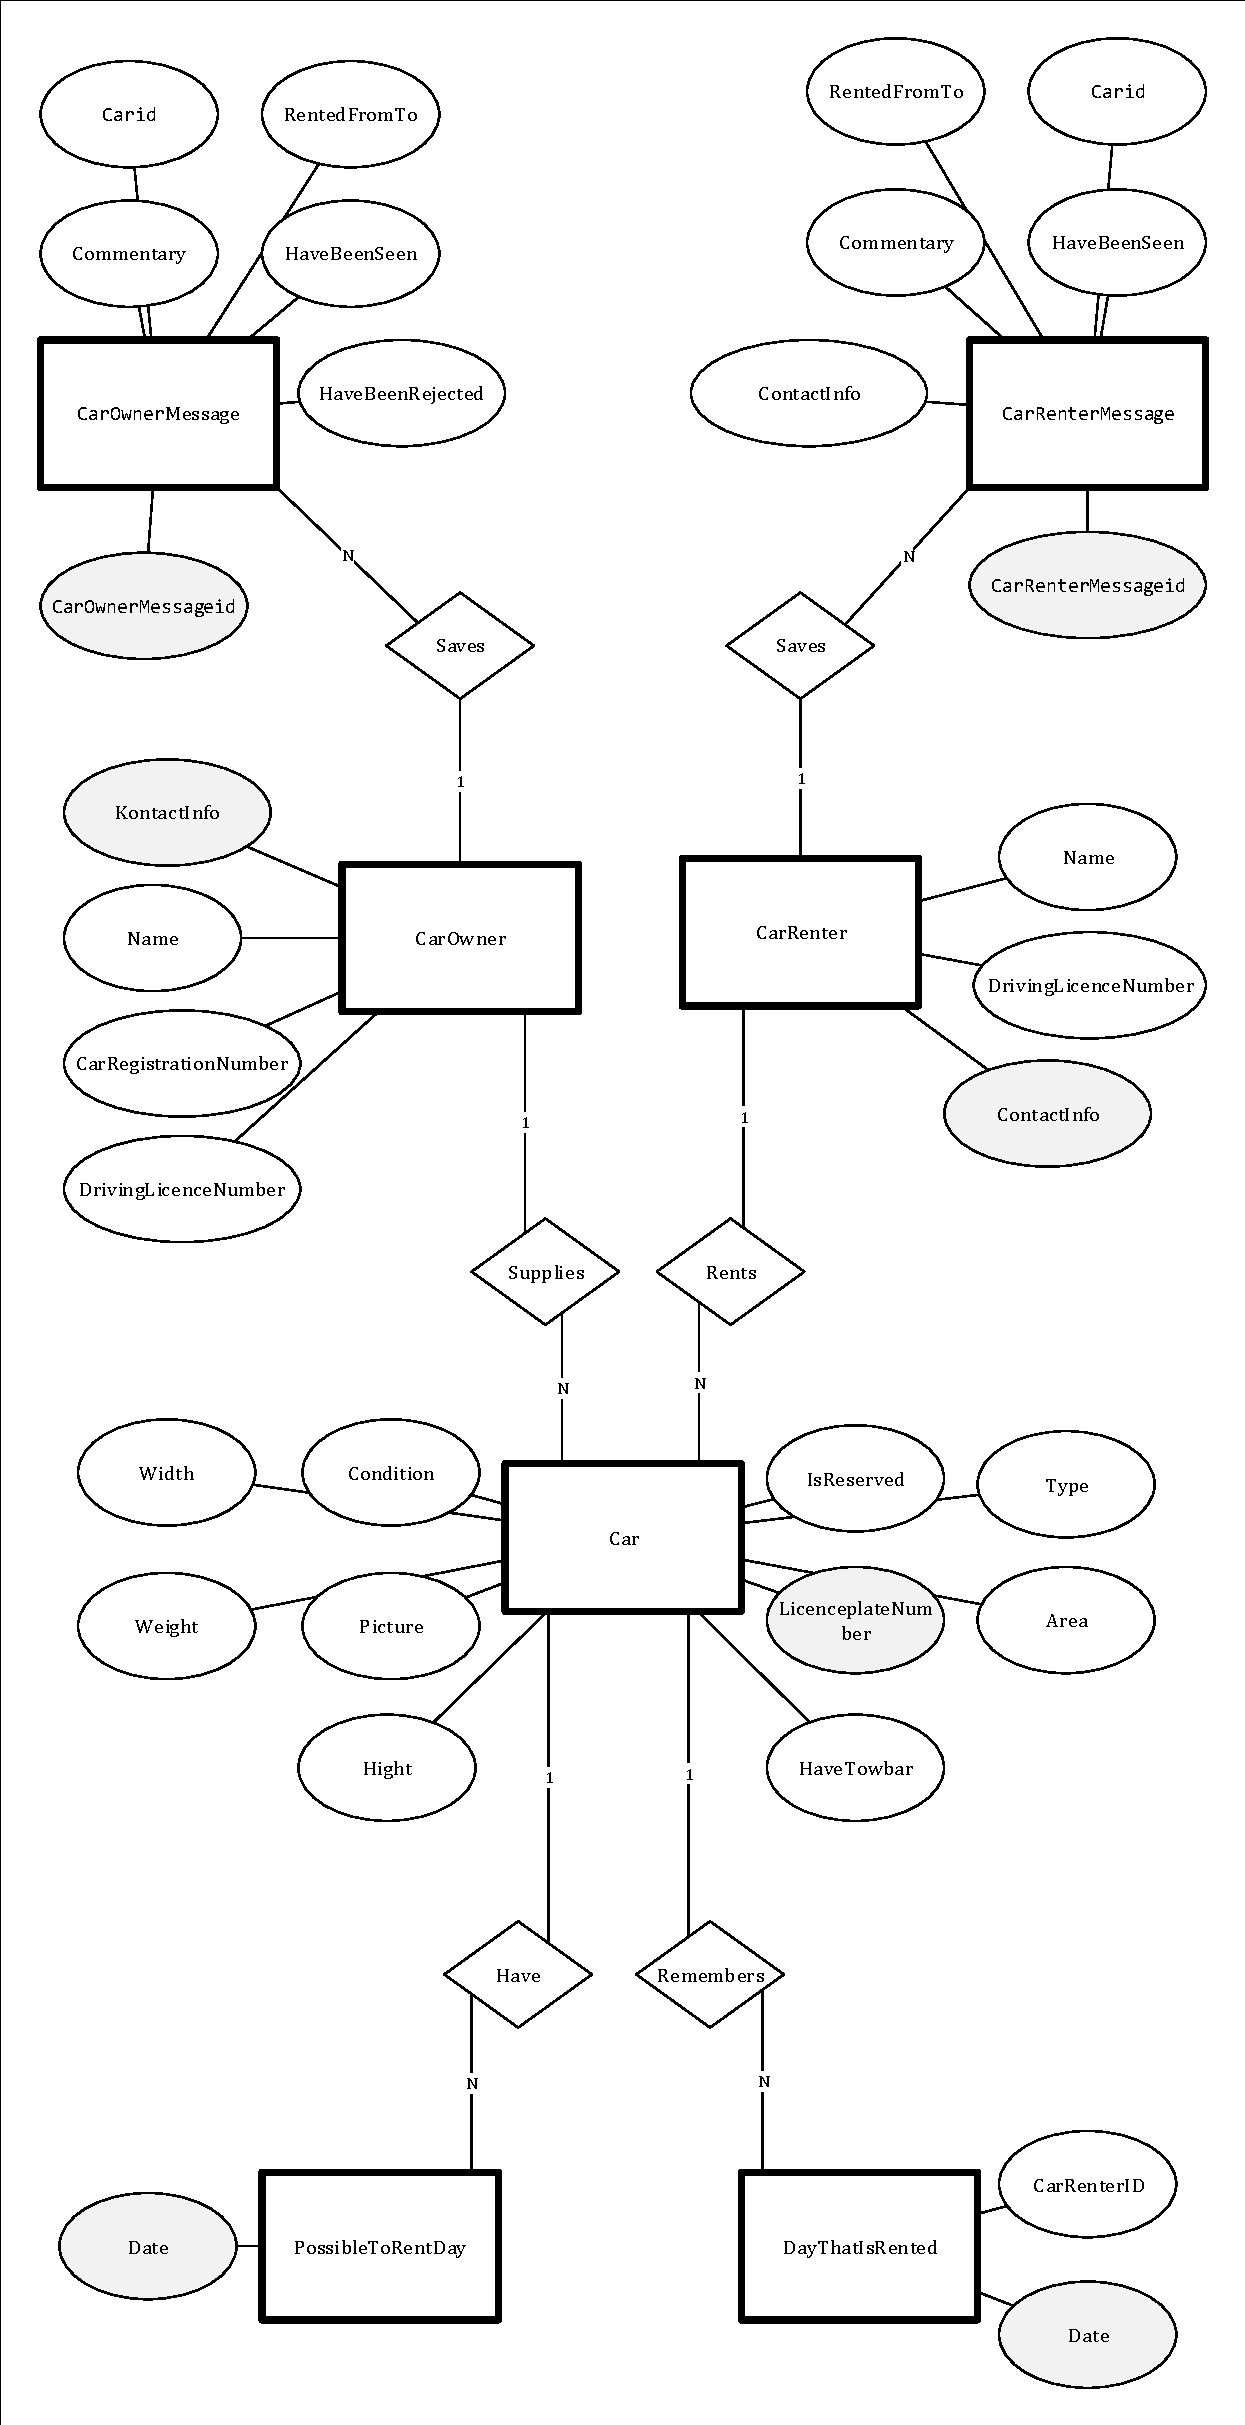
\includegraphics[width=0.9\textwidth]{Arkitektur/Softwarearkitektur/Database/graphics/ER.pdf}
    \caption{Entity–relationship diagram for CarnGo databasen. E/R diagrammet er designet ud fra Chens notation}
    \label{fig:ERDiagram}
\end{figure}
\noindent Databasen ligger på en ekstern server stillet til rådighed af Microsoft Azures cloudplatform. Databasen tilgås med SQL server queries, som automatisk genereres af frameworket (EF core). \\\\
Designet af databasen fokuserer på at optimerer udnyttelse af databasens kapacitet. Det tager betydeligt mere tid at query mindre instanser, da det ofte kræver en del query operationer. Her favoriserer systemet større query operationer, da alle instanserne er ofte tæt beslægtet i forhold til systemfunktionalitet. Det belaster også trådsystemet, da hvert query benytter en separat tråd. I forlængelse af dette prioriteres lokalt modificering (i selve WPF applikationen) indtil alle ændringer er færdig - så samles ændringerne i en større query til databasen. Dette skaber dog også udfordringer i forhold til synkronisering af applikation og database. En ny bil kan være sat til leje i applikationskatologet, hvor to brugere udforsker applikationskataloget og den ene vælger bilen (og dermed være utilgængelig). Her vil den grafiske brugeroverflade ikke være synkroniseret med den anden bruger, og informationen fremvist brugeren er misvisende. Udfordringen er hvornår og hvor tit data skal opdateres i WPF applikationen i forhold til det som findes i databasen. \\\\
En løsning til dette problem kunne være at tjekke databasen oftere end brugeren kan læse data fra skærmen, og derved have en fuldt synkroniseret GUI. Dette ville dog belaste systemet i forhold til antallet af queries, som skal foretages (Nærmest konstant polling af databasen). Det vælges derfor et specifikt tidsinterval på 5 min mellem hvert synkroniseringsevent. Dette er dog ikke helt nok, da der stadigvæk kan opstå misvisende data idet brugeren skifter vinduer i applikationen. Når brugeren navigere mellem vinduerne, sendes et event. Dette event indikerer til vinduet, at det skal opdaterer alt dets data og query efter eventuel nye - det er således selvregulerende i forhold til brugerens aktivitet. \\\\


\end{document}